\documentclass[addpoints,12pt]{exam}
%\documentclass[12pt]{article}
\usepackage[letterpaper, margin=0.75in]{geometry}
\usepackage{graphicx}
\usepackage{enumitem}
\usepackage{booktabs}

\begin{document}
\footer{}{Page \thepage\ of \numpages}{}

\begin{flushright}
\makebox[0.5\textwidth]{\large Name:\enspace\hrulefill}
\vspace{0.2in}

\makebox[0.5\textwidth]{\large Date:\enspace\hrulefill}
\end{flushright}

\begin{center}

\includegraphics[width=10cm]{../images/logo.png}
\end{center}

\begin{center}
\noindent{\LARGE Conceptual Physics \\ Reading Quiz 6}
\end{center}

\noindent\begin{large}\textbf{Due Date: April 6 (before class)}\end{large}
\vspace{0.2in}

This reading assignment covers the material that we will discuss and work on next week. Our class activities will \textbf{assume} that you have read the assigned material, therefore it is \textbf{very important} that you do so to get the most out of the class!

If you did not read all of \textit{The Four Fundamental Interactions} in the course reader, I advise you finish the reading now, particularly the section which discusses carrier particles.

Also below is a cartoon picture of the atom, following the Bohr-Rutherford model that makes it look like planets:

\noindent \begin{center}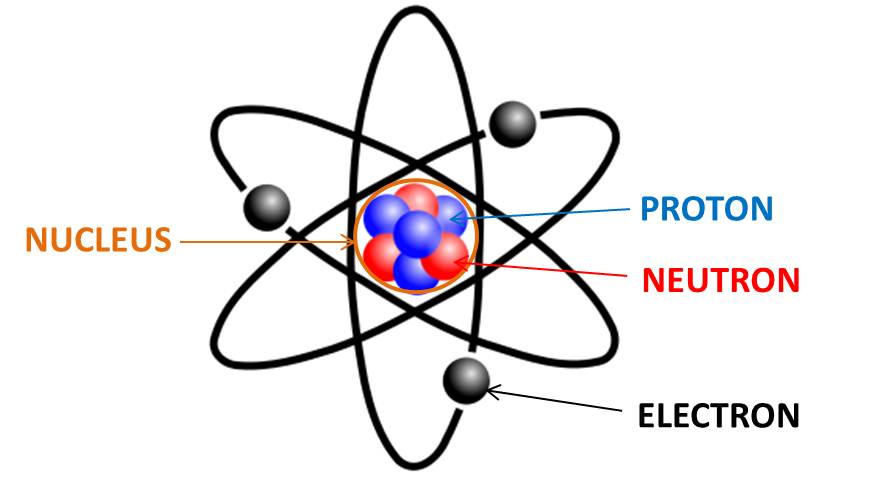
\includegraphics[width=4in]{../images/atom.jpg}\end{center}

Where the \textit{nucleus} is located in the middle of the atom and is orbited by electrons. Protons are \textit{POSIT}ively charged, neutrons carry no charge (\textit{NEUT}ral) and electron are negatively charged (and named for archaic reasons having to due with Greeks and tree resin). Electrons are \textit{fundamental particles} - they cannot (to our knowledge) be further broken down. Protons and neutron, however, are composite particles, meaning that they can be further broken down. \textit{Quarks} come together to form protons and neutrons, and are themselves fundamental particles (discussed in Chapter 0 of \textit{Light and Matter} and chapter 33, section 5 of \textit{College Physics}).

\begin{enumerate}


	\item \textit{Light and Matter} Chapter 17 (Section 1)
	
	Next class we will be discussing light as a wave, and so section 1 of this chapter will be very useful for introducing terminology (frequency, period, amplitude) of waves and oscillations. Both light and sound can be thought of as waves (light as a wave of electric and magnetic fields, sound as a wave in air), and so terminology for the two will be mixed in together in this section and may be confusing.	
	
	\item \textit{Light and Matter} Chapter 19 (Sections 3 and 4)
	
	There is a lot of technical language in sections 1 and 2, although I would encourage you to read them if you are interested. There is a section that uses calculus and is in no way needed for this course. Section 3 provides a useful discussion of light and sound waves, and describes the relationship between waves and the way they travel. Superposition of waves means that, when they overlap, they will either add together or cancel each other out - they do not repel each other (imagine ocean waves - if two come together you get more complex ripples in water, not a repulsion of the waves from each other). If you want to read ahead, section 5 on the Doppler effect will be very useful when we talk about relativity in week 11 and 12.
	
	\item \textit{Light and Matter} Chapter 26 (Sections 1 and 4)
	
	You do not need to memorize the periodic table, however do understand what the different numbers mean. The table that discusses the relative masses with hydrogen close to 1 is in \textit{atomic units}, which are essentially the size of 1 proton (or neutron).
	
	There is a lot of history in this chapter, and I encourage you to read it for your own benefit (but you will not be tested on). Please pay particular attention to the part in section 4 that discusses the structure of nuclei.
	
	
	
	
\end{enumerate}

As part of the reading, please complete the pre-class quiz \textit{before} coming to class. They will be collected at the very beginning.
 
\clearpage

\begin{flushright}
Score: \hspace{0.2in} / \numpoints ~ points
\end{flushright}

\noindent Questions from \textit{Light and Matter} Chapter 17

\begin{questions}

\question[1]
The time required for one repetition of periodic motion is called what?
\fillwithlines{0.5in}

\question[1]
The number of vibrations per second is called what?
\fillwithlines{0.5in}

\question[1]
What term is used to describe how big vibrations are?
\fillwithlines{0.5in}


\end{questions}

\noindent Questions from \textit{Light and Matter} Chapter 19

\begin{questions}

\question[1]
It was thought that light needed a medium through which to travel, just as sound travels through air. For a long time, physicists assumed the existence of a medium for light that would explain how it was able to travel in the vacuum of space (later proved to not exist). What was this medium called?
\fillwithlines{0.5in}

\question[1]
Different frequencies of light correspond with different colors. Is violet high or low frequency light?
\fillwithlines{0.5in}

\question[1]
What is the term used to describe the distance spanned by one repetition?
\fillwithlines{0.5in}

\question[1]
Write down an equation for the speed of a wave, using $\lambda$ and $T$.
\fillwithlines{0.5in}

\end{questions}

\noindent Questions from \textit{Light and Matter} Chapter 26

\begin{questions}

\question[1]
Where in the atom is all the positive charge located?
\fillwithlines{0.5in}

\question[1]
What defines the atomic number of an element?
\fillwithlines{0.5in}

\question[1]
What is an isotope?
\fillwithlines{0.5in}

\end{questions}

\end{document}